\chapter{Design} \label{chp:design}

\section{Introduction}
This chapter will go through the design of a \program{Publisher} and \program{Subcriber} that fulfils the requirements listed in table \ref{tab:requirements}.
At first, this chapter will go through the \textit{Design Requirements} in section \ref{sec:design:requirements} which list the design principles used in this chapter.
In section \ref{sec:design:vcs} a \ac{VCS} is explained, as a \ac{VCS} has similar functionality, as described in section~\ref{sec:streamingidea}.
From the \ac{VCS}, the most widely-used protocols are explained in sections \cref{test, test1, test2}.
At last, the protocols are compared to the requirements from section \ref{sec:analysis:requirements}, in order to find the most suitable protocols.
This chapter will then end up with a list of design choices and requirements for the implementation.

\section{Design Requirements} \label{sec:design:requirements}
The proposed system will be designed using the summarized UNIX philosophy formulated by Doug McIlroy\footnote{\url{https://en.wikipedia.org/wiki/Unix_philosophy\#Doug_McIlroy_on_Unix_programming}}.  
\begin{enumerate}
	\item Programs should do one thing, and do it well.
	\item Programs should be able to work together.
	\item Programs should be capable of taking streams (of text) as input.
\end{enumerate}

Furthermore, the following paramount precepts formulated by Mike Gancarz\footnote{\url{https://en.wikipedia.org/wiki/Unix_philosophy\#Mike_Gancarz:_The_UNIX_Philosophy}} should be used as well.
\begin{enumerate}
	\item Small is beautiful.
	\item Make each program do one thing well.
	\item Build a prototype as soon as possible.
	\item Choose portability over efficiency.
	\item Store data in flat text files.
	\item Use software leverage to your advantage.
	\item Use shell scripts to increase leverage and portability.
	\item Avoid captive user interfaces.
	\item Make every program a filter.
\end{enumerate}

At last, the following requirements should be used.


\begin{enumerate}
	\item Maintainability:
As other people might want to add functionality to the system in the future, it should have high maintainability. This will happen automatically if the ``UNIX design rules'' are kept in mind during design and development.
\item Modular:
The system should consist of multiple small programs which can be used in all existing use-cases but also those that might come in the future.
\item Reusable:
As much code should be as reusable as possible in order to avoid implementing the same functionality multiple times.

    \item Linux utilities should be used as much as possible.
\end{enumerate}

However, splitting functionality into multiple modules should be be done with caution as it might come with the price of performance. Each time programs are split up, there is usually required some communication between the programs or some exchange of memory. The communication might turn out to be unnecessary performance consumption. Therefore splitting programs up is seen as a trade-off between simplicity and performance.

%\todo{a trade-off between simplicity vs. performance}


%By complying with the three ideas from above, the system should consist of small programs that can be put together in different ways to serve different purposes.

%Since the system is developed for biologists, it should be easy to use and require minimum intervention to get it running. Ideally the system should be “plug and play” such that biologists can take the number of recording boxes required for their application and put it all together without the need to configure software on any of the boxes. \todo{Add Extensibility somewhere, maybe not due to maintainability}

%\todo{Add: Write as little code as possible, use already existing code maintained by other developers}
%\todo{add: Should be a requirement that it should be easy to write new nodes. Should not require an interface to send commands, should be self-contained as possible.}

%\todo{Design inspired by Daniel J. Bernstein, software run in "chains"}
%Furthermore the system should also be:





\section{Video Conference System(VCS)} \label{sec:design:vcs}
% http://www.faqs.org/rfcs/rfc5219.html <- mp3 i rtp
% RTP description https://flylib.com/books/en/4.245.1.27/1/
\ac{VCS} utilize audio and video streams, as a video conference is a connection between people residing in separate locations. This connection gives the impression that people participating in the video conference are present in the physical meeting. VCS usually allows for multiple participants to join a meeting where all participants are able to see each other. VCS might allow control of the camera by the remote participant in order to look at the person who is currently speaking. 
Lip-sync is often preferred during the video conference, to further give the impression the remote-participant is present. Lip-sync is when the sound from the remote participants is synchronized with the video stream. This usually has to be implemented by the streaming protocols as sound and video is not necessarily transmitted in the same stream and so are not synchronized when received by the recipient.

\begin{figure}[H]
	\centering
	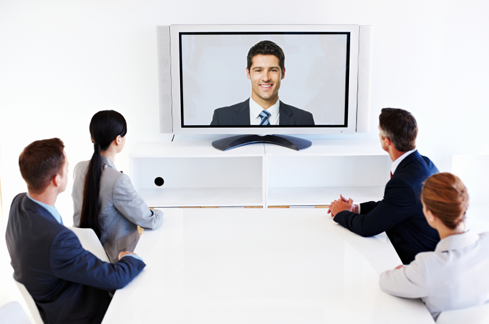
\includegraphics[width=0.8\textwidth]{figures/vcs_overview.png}
	\caption{Example of a video conference system where five people are participating in a meeting, but the third person is not physically present.} \label{fig:design:vcs}
\end{figure}

\ac{VCS} works similarly to \ac{VoIP}, which is like a conference system between two participants only using sound. A typical protocol stack is shown in figure~\ref{fig:design:protocolstack}. 

%rtcp used to adjust codec wrt. bandwidth
\begin{figure}[H]
	\centering
	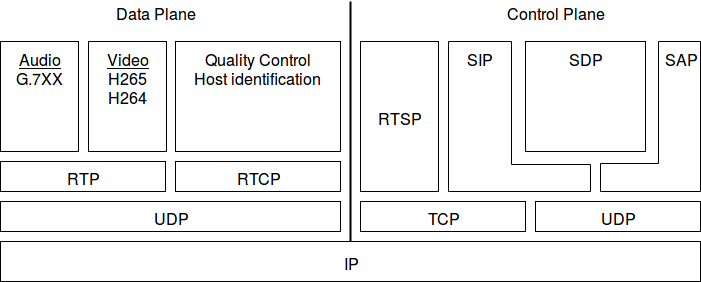
\includegraphics[width=\textwidth]{figures/protocol_stack}
	\caption{Protocols used in VCS and VoIP. It should be noted, that not all protocols necessarily are used at the same time. The figure is inspired by \url{https://commons.wikimedia.org/wiki/File:SIP_protocol_stack.svg}
	\label{fig:design:protocolstack}
\end{figure} 

Figure \ref{fig:design:protocolstack} shows how the protocols stack on top of each other, where IP is in the bottom layer in the \textit{Data Plane} and \textit{Control Plane}. The  \textit{Data Plane} is where the encoded audio and video is transferred, between participating nodes. Part of the \textit{Data Plane} is also the RTCP protcol, which provides channel information about the quality between participants. Usually the RTP protocol is used to packetize encoded audio and video - encoding is handled by G.7XX or H264/H265. The \textit{Control Plane} is where sessions are initiated. In VoIP, \ac{SIP} is usually used to initiate sessions, but other protocols such as RTSP and SAP can be used as well. Which protocol is used to initiate the session depends on the application and whether it is a session between multicast participants or unicast. SDP is used in \ac{SIP} to negotiate supported codecs between sender and receivers, but used in RTSP and SAP to describe a session with encoding statically set by the session originator\citep{voip_fundamentals}.  \ac{SIP} is not further described, as the protocol is relevant for this application, as multicast groups and not unicast is used. 

The protocols in figure \ref{fig:design:protocolstack} are listed in table~\ref{tab:design:protocollist}. Proprietary VCSs such as Skype use closed protocol specifications which are not included in the table.


\begin{table}[H]
	\centering
	\resizebox{\textwidth}{!}{%
		\begin{tabular}{@{}|l|l|l|l|@{}}
			\toprule
			\textbf{Protocol}              & \textbf{Described in} & \textbf{Functionality} \\ \midrule
			Real time Transport Protocol (RTP)    & \ref{sec:design:rtp}                  & Transports video, sound etc.\\ \midrule
			Real time Control Protocol (RTCP)          & \ref{sec:design:rtcp}                & Quality feedback, participant ident. and timing\\ \midrule
			Session Description Protocol (SDP)   & \ref{sec:design:sdp}                  & Describes a RTP session\\ \midrule
			Session Announcement Protocol (SAP)  & \ref{sec:design:sap}                  & Announces a SDP on multicast group\\ \midrule
			Real Time Streaming Protocol (RTSP) & \ref{sec:design:rtsp} & Creates session \\ \bottomrule
		\end{tabular}%
	}
	\caption{Table shows protocols often used in video conference systems}
	\label{tab:design:protocollist} 
\end{table}
\todo{Add RFC to table for each protocol}

\todo{Add RTSP and other non-relevant protocols?}

\subsection{Real-time Transport Protocol} \label{sec:design:rtp}
The RTP protocol is a network protocol for transmitting media such as audio, video and text in streaming applications such as \ac{VoIP} and video conference systems. The terminology used throughout the thesis is from RFC7656\citep{RFC7656}. Not all terms defined in RFC7656 are used in attempt to limited the scope of the RTP terminology used in this thesis. Details are the RTP protocol is from RFC3550\citep{RFC3550}.

The RTP protocol does not specify how the data should be packet into the payload of an RTP packet. This is defined by profiles and packet types. A profile can contain multiple data formats, and might describe some general details about the content of the RTP packet.
The most used profile is the ``RTP/AV audio video for conference with minimal control'', which is used for streaming audio and video witch is described in section \ref{sec:design:profile}.

\myparagraph{RTP Stream} \label{sec:design:rtpstream}
RTP packets are sent in RTP streams. An RTP stream corresponds to a source stream as introduced in section \ref{sec:analysis:pubsub}. RTP is usually run over UDP, but it can be used over TCP as well. RTP is typically used with port 5004, but 5004 is not assigned to RTP by IANA\citep{iana_ports}.


\myparagraph{RTP Session} \label{sec:design:rtpsession}
An RTP Session is a group of participants communication using RTP.
An RTP stream is sent in a RTP session, such that participants in that session receive the RTP stream. An RTP session can potentially carry multiple RTP streams. Within an RTP session, every participant can find metadata and control information (over RTCP) about all the RTP streams in the RTP session. A participant can be involved in multiple RTP sessions e.g. when a participant receive more than one media. In RTP sessions, each media is typically carried in a separate RTP session with its own RTCP packets unless the the encoding itself multiplexes multiple media into a single data stream. See RTCP packets in section \ref{sec:design:rtcp}. Multiple RTP sessions are usually referred to as a multimedia session.


An RTP session can be identified in two ways:
\begin{itemize}
	\item In unicast with e.g. two participants talking to each other, an RTP session is defined as two destination transport addresses, each with a port pair for RTP and RTCP. This allows both participants to send RTP and RTCP packets to each other.
	\item In multicast with N participants, an RTP session is defined as a destination transport address and a port pair. This allows multiple participants to send and receive RTP streams by sending and receiving from the multicast address.
\end{itemize}


Figure  \ref{fig:design:rtp:session} shows an illustration of a RTP session with two RTP session in a multicast group.
\begin{figure}[H]
	\centering
	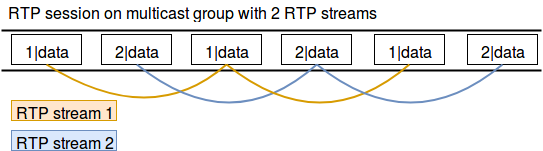
\includegraphics[width=\textwidth]{figures/rtp-session}
	\caption{Shows an illustration of an RTP session with two RTP streams. Each color represent a RTP stream. It should be noted that the packets are interleaved; however, this is just an example, as the RTP packets might not come with same frequency in an RTP session.} \label{fig:desion:rtp:session}
\end{figure}

\myparagraph{RTP Packet}
An RTP packet is depicted in figure~\ref{fig:design:rtppacket}. The static RTP header is 12 bytes, when no CSRC is present and no additional headers.
\todo{Describe CSRC + header extensions}

\begin{figure}[H]
\centering
\begin{verbatim}
0                   1                   2                   3
0 1 2 3 4 5 6 7 8 9 0 1 2 3 4 5 6 7 8 9 0 1 2 3 4 5 6 7 8 9 0 1
+-+-+-+-+-+-+-+-+-+-+-+-+-+-+-+-+-+-+-+-+-+-+-+-+-+-+-+-+-+-+-+-+
|V=2|P|X|  CC   |M|     PT      |       sequence number         |
+-+-+-+-+-+-+-+-+-+-+-+-+-+-+-+-+-+-+-+-+-+-+-+-+-+-+-+-+-+-+-+-+
|                           timestamp                           |
+-+-+-+-+-+-+-+-+-+-+-+-+-+-+-+-+-+-+-+-+-+-+-+-+-+-+-+-+-+-+-+-+
|           synchronization source (SSRC) identifier            |
+=+=+=+=+=+=+=+=+=+=+=+=+=+=+=+=+=+=+=+=+=+=+=+=+=+=+=+=+=+=+=+=+
|            contributing source (CSRC) identifiers             |
|                             ....                              |
+-+-+-+-+-+-+-+-+-+-+-+-+-+-+-+-+-+-+-+-+-+-+-+-+-+-+-+-+-+-+-+-+
|                             Payload                           |
|                              ....                             |
|                              ....                             |
+-+-+-+-+-+-+-+-+-+-+-+-+-+-+-+-+-+-+-+-+-+-+-+-+-+-+-+-+-+-+-+-+
\end{verbatim}
\caption{Figure of how the RTP packet is structured\citep{RFC3550}}
\label{fig:design:rtppacket}
\end{figure}

\myparagraph{Payload}
\myparagraph{SSRC}
The \ac{SSRC} field is a 32 bits identifier that uniquely identifies a participant within an RTP session. All RTP and RTCP packets sent by a participant in an RTP session carries the same SSRC, such that receiving participants know where a RTP or RTCP packet belongs to. In case a property change of a RTP stream such as encoding, the SSRC must change such that receiving participants is aware of the property change.

\myparagraph{Timestamp}
The timestamp is a 32 bit NTP timestamp with random offset that reflects the sampling instant of the first octet in the RTP packet. Multiple consequence, logically generated at once, RTP packets can have the same timestamp, in case the payload of multiple RTP packets are related such as in a video frame.
The timestamp is also used to synchronize multiple RTP streams and to estimate jitter in order to provide quality feedback to the sender using RTCP RR as described in section~\ref{sec:design:rtcp}.
As the clock frequency is dependent on the content of the RTP packet, the clock frequency is specified in the payload specification. This is usually specified in a SDP as described in section~\ref{sec:design:sdp}. As an example, for fixed-rate audio the timestamp clock would likely increment by one for each sampling period. If an audio application reads blocks covering 160 sampling periods from the input device, the timestamp would be increased by 160 for each such block\citep{RFC3550}.

To synchronize a single RTP stream, the timestamp can be used however; if multiple RTP streams should be synchronized e.g. in the case of video and audio, the timestamps are not enough, as they may advance at different speeds with different offsets. The timestamp is then used together with RTCP SR packets, with associates the timestamp with a 64 bit NTP timestamp. The RTCP SR packet is usually sent with a lower frequency than the 32 bit timestamp. The 64 bit reference clock is shared between multiple media streams to be synchronized. The RTCP SR packet is described in section~\ref{sec:design:rtcp}.


\myparagraph{Sequence Number}
The sequence number is a 16 bit integer that can be used by receiving participants to estimate the packet loss. This value must be randomly initialized.

\myparagraph{Payload}
The payload is the content of the RTP packet. This is the encoded media such as audio or video. 

\myparagraph{Packet Type}
The packet type identifies the format of the payload. RFC3550 does not define which values that can be used.


\myparagraph{Mark bit}
The mark bit can be used to signal significant events. RFC3550 does not specify how this bit should be used.

\todo{RTP supports header extentions}
\todo{Verify clockrate(timestamp) is in order with RTP packet timestamp description}


\subsection{Real-time Control Protocol} \label{sec:design:rtcp}
RTCP runs alongside RTP and provides periodic metainformation about an RTP stream. RTCP is usually sent over UDP, 1 port higher than RTP but can be sent over TCP at a random port. The primary function is to provide feedback on the quality of the data distributed. RTCP is also used to provide participant identification, synchronization between RTP streams and membership management. Feedback quality information is used in unicast applications to adopt the encoding to each receiver. The receiving participant can keep track of the number of lost packets and provide feedback to the sender, which allows the sender to change the encoding. This is useful if the bandwidth between a sender and receiving participant is limited.  Although RTP packets are typically sent in the microsecond scale, RTCP operates on the scale of seconds.
For all participants, RTCP provides identification using a unique \ac{CNAME}.
Since the RTP SSRC identifier may change if a conflict is discovered or a property of an RTP stream changes, participants use the CNAME to keep track of each participant. Using the \ac{CNAME} and other information, participants are aware of all participants in an RTP session.
The information sent in RTCP is also necessary for synchronization between RTP streams e.g. lip synchronization between RTP streams carrying audio and video.

An example of a the RTCP packets structure is depicted in figure \ref{fig:design:rtcp:packet}.
\afterpage{
	\begin{figure}[H]
		\begin{center}
			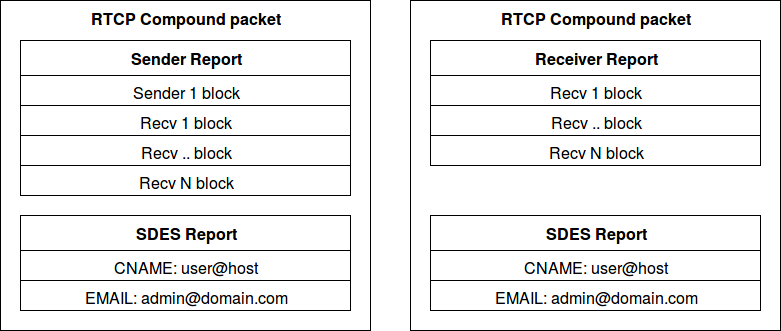
\includegraphics[width=1\textwidth]{figures/rtcp_blocks_compound}
			\caption[okok]{Figure shows 2 examples of RTCP compound packets. The left figure shows an RTCP compound packet with a SR and SDES packet, the right shows the same but with a RR instead of the SR \footnotemark } \label{fig:design:rtcp:packet}
		\end{center}
	\end{figure}
  \footnotetext{The figure is made by thorough reading of RFC3550}
}

From figure \ref{fig:design:rtcp:packet} it can be seen, how multiple RTCP messages are concatenated into a compound packet. Each packet type has its own header; however, they all follow the same number of fields, and size of each field though have different names. The packets are packet into a compound packet such that each participant emits all his packets at the same time. As the length of each message type is present, the packets can be extracted from the compound packet. The reason to compound packets is due to an algorithm that based on different parameters such as the number or participants, calculates how often compound packets should be sent.\footnote{\url{https://tools.ietf.org/html/rfc3550\#section-6.3.1}}

The RTCP protocol contains the following 5 packet types:
\begin{itemize}
	\itemmsg{Sender Report(SR)}: The sender Report (Packet Type = 200) is periodically sent by sending participants in a RTP session. It contains an absolute 64 bit NTP timestamp which is used to synchronize RTP streams. The 32 bit timestamp from the RTP packet is also included, in order to associate the 64 bit timestamp to the RTP packet. Further more the SR contains a packet and octet count, such that the receiving participant can calculate lost RTP packets. After the SR, an RR (See next item) can be added to the compound packet.

	\itemmsg{Receiver Report(RR)}: The RR (Packet Type = 201) is for participants receiving RTP streams. The RR contains information about packet lost, jitter, when the last SR was sent etc. This information can be used by the sender to adjust the encoding to reduce the packet loss. Each RR can contain multiple receive blocks, as depicted in figure \ref{fig:design:rtcp:packet}

	\itemmsg{Source Description(SDES)}: The Source Description (Packet Type = 202) is used to provide UTF8 encoded information about a participant. The only mandatory information is the \ac(CNAME), but name, email, telephone number can be provided as well. The CNAME is not changing such that the sender can be identified if the SSRC changes. The CNAME is usually comprised of the host's username and hostname. The SDES packet allows for application specific extensions. 

	\itemmsg{Goodbye (BYE)}: The Goodbye (Packet Type = 203) is used by participants to signal they are leaving the RTP Session. 
	
	\itemmsg{Application-Defined(App)}: The App (Packet Type = 204) is intended for experimental use without applying for new packet types. This packet has a subtype-field that allows defining types of the APP packet. 
\end{itemize}

Each of the messages types are processed independently.
A compound packet must obey the following constrains:

\begin{itemize}     
    \item An SDES packet containing a CNAME item must be included in each compound RTCP packet. Other source description items may optionally be included if required by an application. \footnote{\url{https://tools.ietf.org/html/rfc3550\#section-6.1}}
      
    \item Other RTCP packet types, including those yet to be defined, may follow in any order, except that BYE should be the last packet sent with a given SSRC. Packet types may appear more than once. \footnote{\url{https://tools.ietf.org/html/rfc3550\#section-6.1}}
\end{itemize}


\subsubsection{Profile} \label{sec:design:profile}
RTP and RTCP leaves out details about how streams should be encoded in order to be general media transport purpose protocols. Details like this are specified in a profile. A profile also allows for header extensions added to the RTP and RTCP packets.\todo{Write this better}


%Examples of questions answered by profiles are listed below.
%\begin{itemize}
%	\item How encoded media is mapped into the \textit{Packet Type}-field in the RTP header
%	\item How often RTCP Sender-Reports and Recever-Reports should be sent.
%	\item How audio and video should be packet into a stream e.g. How to know which channel a sample belongs to.
%	\item Calculation of the clock rate in \textit{Timestamp}-field.
%	\item The semantics of the \textit{Marker}-bit.
%\end{itemize}

%Profiles answer the questions listed above, and many more details regarding RTP and RTCP. 
At the moment of writing, four profiles are available. These are listed below:

\begin{itemize}
	\item RTP profile for audio and video Conferences with monimal control (RFC3551)
	\item The secure Real-time Transport Protocol(RFC3711) \footnote{\url{https://tools.ietf.org/html/rfc3711}}
	\item RTP audio-visual profile with feedback (RFC4585)
	\item Extended secure RTP profile for RTCP-based feedback(RFC5124) \footnote{\url{https://tools.ietf.org/html/rfc5124}}
\end{itemize} \citep{johnston2004sip}

\textit{The secure Real-time Transport Protocol} and \textit{Extended secure RTP profile for RTCP-based feedback} decribes how the content of RTP streams can be encrypted.

\textit{RTP audio-visual profile with feedback} is an extension to the Audio/Video profile where it changes the retransmission algorithm of RTCP reports in order to make the sender change the encoder faster using timely feedback. \citep{RFC4585}

Generally, the \textit{RTP Profile for Audio and Video Conferences with Minimal Control}\citep{RFC3551}(Audio/Video) profile is used in audio and video systems.\citep{perkins2003rtp}.
Three of the parameters defined by the Audio/Video profile is listed below.
\begin{itemize}
	\item UDP isused for underlaying transport
	\item RTP port numbers are always even - the corresponding RTCP port is the next highest port, which is always an odd number
	\item No header extensions are used
\end{itemize} \citep{johnston2004sip}

The Audio/Video profile specifies different \textit{Payload Formats} that can be used in the RTP stream. Initially the Audio/Video profile should define all encodings available, but later it was discovered to be easier to reserve a range of dynamic types, such that the profile didn't have to define all possible encodings. If a dynamic type is chosen, the SDP provides the properties of the stream such as encoding, sample size, bitrate, number of channels etc. such that the receiving participants know how to interpret the stream.
The SDP is described in section \ref{sec:design:sdp}.

In the Audio/Video profile, the \textit{Marker}-bit is used to signal a talkspurt after a long period of silence. The Audio/video profile then denotes how this can be used to adjust network delay.

\subsection{Session Description Protocol} \label{sec:design:sdp}
The Session Description Protocol(SDP) is a protocol for describing RTP streams.
SDP does not provide any media nor specify how the SDP must be transferred.
SDP is widely used in VoIP and conference systems, where parameters must be known to receivers before the RTP streams can be decoded and presented.
In multicast systems, SDP is also used to announce streams such that receivers know which multicast group to join in order to get the streams. Usually the SDP is sent from the originator of the session, but SDP can also be used to negotiate parameters between originator and participants.
In general, the SDP must provide enough information about a stream such that a participant can decide whether the stream should be joined or not.
SDP is designed to be extensible to support new media types and formats.
If a dynamic packet-type is chosen in the audio/video profile, SDP supports adding additional information to the session description. 

An SDP file comprises a number of strictly defined key-value pairs.
The SDP describes several keys where some must be provided and others are optional.
A key-value pair is defined as shown below:
\begin{verbatim}
<key>=<value>
\end{verbatim}

No spaces are allowed around the key or value.
The order of the keys are dictated by the RFC. The reason for the strict format is to ease parsing and to easily detect errors in an SDP file. An example of an SDP is shown below:

\begin{verbatim}
    v=0
    o=jdoe 2890844526 2890842807 IN IP4 10.47.16.5
    s=SDP Seminar
    i=A Seminar on the session description protocol
    u=http://www.example.com/seminars/sdp.pdf
    e=j.doe@example.com (Jane Doe)
    c=IN IP4 224.2.17.12/127
    t=2873397496 2873404696
    a=recvonly
    m=audio 49170 RTP/AVP 96
    a=rtpmap:96 L8/8000
\end{verbatim}
The keys used above are described below in the list below. \\
\textbf{v=} Version. Currently only version 0 exists. \\
\textbf{o=} Originator, information about who sends the streams. Source IP, sessionid etc. \\
\textbf{s=} Session name. \\
\textbf{i=} Session Information \\
\textbf{u=} Url to more information about the session.\\
\textbf{e=} Email address of originator.\\
\textbf{c=} Connection data comprising of ``nettype'' ``addrtype'' ``connection-address''.
\begin{itemize}
	\item The first field ``nettype'' is the network type where only Internet is defined. 
	\item The second field ``addrtype'' is the type of the address. This can either be IPv4 or IPv6.
	\item The third field ``connection-address'' defines the address participants must connect to in unicast applications and what group participants must join when multicast is used.
\end{itemize}
\textbf{t=} - Timing defines when the stream starts and stops. \\
\textbf{a=} - Attribute used to extend the SDP to support additional properties. Recvonly tells participants to only receive from this session. \\
\textbf{m=} - Media comprising of ``media'' ``port'' ``proto'' ``fmt'' ...
\begin{itemize}
	\item Media defines whether the stream is audio, video, text or application.
	\item Port is where participants must connect to when unicast is used. If multicast, this port is where participants will receive the stream.
	\item Proto is the transport protocol. This is usually RTP/AVP, which means RTP is used with the audio/video profile.
	\item Fmt is application specific. If audio/video profile is chosen, fmt describes the payload-type used in the RTP stream.
\end{itemize}
\textbf{a=} is an additional parameter. rtpmap is used when a dynamic payload type is used in the audio/video profile. rtpmap maps the packet-type to the encoding used of the RTP payload. In the example above, L8 is defined as 8 bit raw sound with sample frequency of 8 khz. Additional arguments can be set by adding a /\textless param\textgreater to the list, such as /2 for stereo.

All key-value pairs above m= applies to all sessions, where key-value pairs below an m= only applies to that particular m=. \todo{Verify this with RFC}

The list of key-value pairs is not exhaustive. SDP supports more keys as described in RFC4566.

%A media is defined as:
%            m=audio 49232 RTP/AVP 0
%            m=audio 1337 RTP/AVP 98
%When a dynamic packet type is in use, the following parameter is given:
%            a=rtpmap:98 L16/16000/2
%This associates the the dynamic payload type, 9, with the encoded format which in this case is L16 with a clock frequency of 16000 stereo.

\subsection{Session Announcement Protocol} \label{sec:design:sap}
The \ac{SAP} protocol is used to advertise multicast RTP sessions. SAP packets are send to a wellknown multicast group that receivers are listening to. When a SAP packet is received, the receiver can join the multicast group to get the announced RTP session. An example is depicted in figure \ref{fig:design:sap}. SAP provides authentication and encryption of sessions announcements such that receivers can authenticate the credibility of teh session announcement. The SAP packet contains a \textit{Message Type}-bit, that being set to 1 means the packet announces the deletion of a packet, if 0 a new session is announced. The payload of the SAP packet is a SDP file describing a RTP session. The SAP packet also contains a hash value of the packet that indicates when a SDP packet has changes such that receivers know when to decrypt and parse the payload. \citep{RFC2974}


\subsection{Real Time Streaming Protocol} \label{sec:design:rtsp}
The RTSP protocol is a network control protocol used to establish and control streams between multiple clients and a server. Clients receiving stream get \ac{VCR}-like command such as Start, Pause etc in order to control streams in real-time. RTSP is only used for control, not for delivering the actual data as this is the responsibility of RTP/RTCP.
RFC2326 describes RTSP but has been deprecated by RTSP v2.0 in RFC7826. RTSP is extensible in that it allows for additional methods and headers to be added.
RTSP is usually used over TCP port 554, which is a wellknown port assigned by IANA.\footnote{\url{https://www.iana.org/assignments/service-names-port-numbers/service-names-port-numbers.xhtml?&page=11}} RTSP is simular to HTTP in that it has headers and a body, and uses methods to call on the server. As opposed to HTTP, RTSP maintains a state by using a \textit{Session} header, followed by unique session identifier.

An example of a RTSP session is depicted in figure \ref{fig:design:rtsp:example}.
\begin{figure}[H]
	\centering
	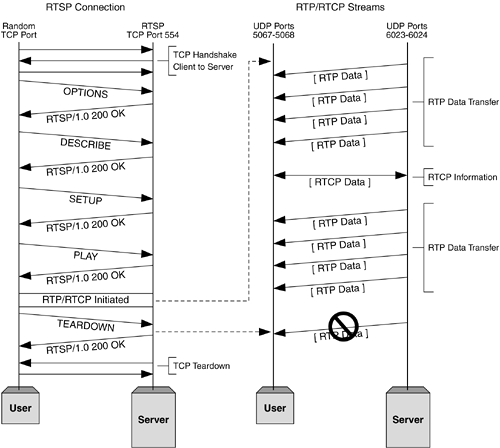
\includegraphics[width=\textwidth]{figures/rtsp_example}
	\caption{Figure of client that interacts with a server. Figure is taken from \url{http://www.informit.com/articles/article.aspx?p=169578&seqNum=3}}
	\label{fig:design:rtsp:example}
\end{figure}

In figure \ref{fig:design:rtsp:example}, an example of a client requesting a stream from a server is shown. As RTSP is run over TCP in the example, a 3-way handshake has to be created before RTSP packets can be sent.
Each of the messages are explained below:
\begin{itemize}
	\item \textbf{OPTIONS} is issued by the client, in order to get information about a stream. The client provides a url to the wanted stream fx. rtsp://example.com/stream.mp4. The server then replies back with "200 OK" if the url exists, and a list of the supported request types such as: Play, pause, teardown etc.
	
	\item \textbf{DESCRIBE} is issued by the client, in order to get a description of the stream. The description is in the SDP format containing information about encoding, bitrate etc. as described in section \ref{sec:design:sdp}.
	
	\item \textbf{SETUP} is issued by the client when the client is ready to configure how the stream should be sent to the client. The client provides two ports in the SETUP request, which denotes the destination port to which the server should send the RTP/RTCP packets.
	
	\item \textbf{PLAY} is issued by the client when the client is ready to get the stream.
When \textbf{PLAY} is received and processed by the server, the server starts to send RTP/RTCP packets to the client to the port provided in the SETUP request.
In order to avoid problems with firewalls between the server and client, the RTP and RTCP packets can be interleaved into the TCP connection created by RTSP.
The \textbf{PLAY} method supports a \textit{range} header, where a range in the stream of the interest can be specified.
The range is used by the client to specify when to see the stream from and to. 
The unit of the range is specified in the \textit{Accept-Ranges} sent in the \textbf{SETUP} method. RFC7826 states, that \ac{NTP} and Absolute Time in ISO8601\footnote{\url{https://www.w3.org/TR/NOTE-datetime}} suporting decimal fractions of seconds, but other units such as bytes\footnote{\url{https://tools.ietf.org/html/rfc7826\#section-18.40}} may be supported as well.
	\item \textbf{TEARDOWN} is issued when the client wants to close the connection. The server will then stop streaming RTP/RTCP, and close the TCP connection.
\end{itemize}

In RTSP v1.0\citep{RFC2326}, two methods are mentioned which have been removed in RTSP v2.0. RTSP v1.0 and v2.0 allow for extension of methods.
\begin{itemize}
	\item \textbf{RECORD} is issued by the client, when it wants to record part of a live stream. A \textit{Conference} header is present, which relates an existing conference such as RTP multicast session and a RTSP session such that the server knows what to record. A \textit{Range} header similar to \textbf{PLAY} is used to specify a range to be recorded.
	\item \textbf{ANNOUNCE} can be issued by both server and clients in order to inform the opposite part of the properties of a RTP stream. If \textbf{ANNOUNCE} is sent from the client to the server, the method is used to tell the server about a new stream that is available. Other clients can then do a \textbf{DESCRIBE} on the newly created URI in order get a session description. If the method is issued by the server, its because the RTP session has changed and the server is pushing out a new session description.
\end{itemize}


\section{Design}
This section presents the design of the streams, metadata \program{Publisher} and \program{subscriber} and \program{Historian} using the requirements from \ref{tab:requirements} to the protocols described in section \ref{sec:design:vcs}. The end of this section will summarize the requirements from the analysis with the protocols.
The final design is depicted in figure \ref{fig:design:overall}.
\begin{figure}[H]
	\centering
	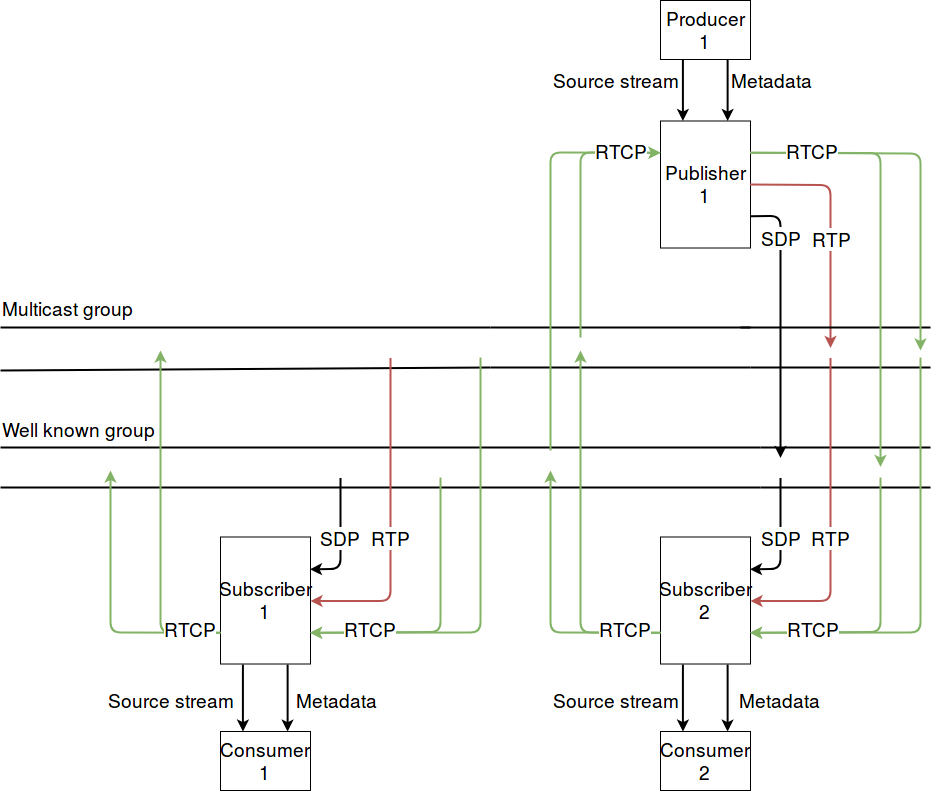
\includegraphics[width=\textwidth]{figures/design_overall.png}
	\caption{The figures shows the final design of the \pubs{} and \subs{}. The figure shows two \pubs{} that have subscribed to the multicast session announced by \textit{Publisher1}. It should be noted that a multicast group will be added for each \pub{} that is run.} \label{fig:design:overall}
\end{figure}

%	\item A stream can be either continuous or discrete.
%	\item A stream must comprise different datatypes only by relying on available codecs.

%   \item Streams must be sent in multicast groups.
%   \item Each must must have its own multicast group.
%	\item A stream must be packet-oriented, stateless and transported over UDP
%	\item A stream must be robust to UDP packets that arrive out of order or never arrive.
%	\item A stream must be represented unambiguously


\subsection{Stream}
\textit{R1: A stream can be either continuous or discrete} \\
Given that the RTP protocol only adds a header to the payload, and that the RTP protocol is agnostic to the payload, RTP does not constrain the payload in any way.\\

\noindent\textit{R2: A stream must comprise different datatypes only by relying on available codecs.}\\
As RTP does not specify how data should be encoded, any type of encoding can be used, as long a codec exists. As profiles exist that specify how sound and video should be encoded and describes such as the Audio/video profile, the RTP protocol with the Audio/video profile should be used to send audio streams. In case of Events, a profile should be define that specifies the semantics of a RTP stream carrying an event. This specification is defind in section \ref{sec:design:metadataprofile}. \\

\noindent\textit{R3: Streams must be sent in multicast groups.}\\
As RTP allows streams to be sent to a multicast group, RTP is suitable for this requirement. \\

\noindent\textit{R4: Each must must have its own multicast group.}\\
Given R3, a stream should be packet into a RTP stream. At it should be possible to only get the data from one stream and not all at once, each RTP stream should be allocated its own RTP Session. This means, an RTP session will only carry one RTP stream with it's associated RTCP traffic. This allows \program{Subscribers} to only receive the stream from the \program{Publisher} of interest without receiving all streams and have to dump those not needed.\\

\noindent\textit{R5: A stream must be packet-oriented, stateless and transported over UDP} \\
Given that RTP packets are transported over UDP, the streams will be packet-oriented and stateless.\\

\noindent\textit{R6: A stream must be robust to UDP packets that arrive out of order or never arrive.} \\
As the RTP header contains a sequence id, the receiver can keep track of how many packets it is missing. As no global information about the stream is carried in the RTP packet, no information is lost, except the payload. If a codec is used that relies on receiving multiple consecutive RTP packets, this will not be the case. Therefore, the RTP packets must not use a codec that expects to receive multiple consecutive RTP packets. \\

\noindent\textit{R7: A stream must be represented unambiguously} \\
As the header contains an SSRC that is unique in a particular RTP session, the stream will be unambiguous with an RTP session. Furthermore, an RTP session will usually be represented either being on a particular port or multicast address.


A source stream, packetized into an RTP stream, in an RTP Session is shown in figure \ref{fig:design:stream}.

\begin{figure}[H]
	\centering
	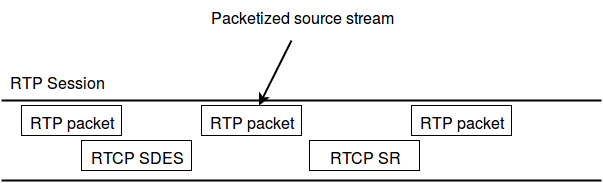
\includegraphics[width=\textwidth]{figures/sourcestream-in-rtp}
	\caption{The figure depicts an packetized source stream packed into RTP packets in an RTP session}
	\label{fig:design:stream}
\end{figure}


%	\item Events must have a start time and date
%	\item Events must have a duration.
%	\item Events must contain data relating to the event.
\subsubsection{Events}
Given that Events are considered packets in a discrete stream, the RTP packet can also be used to transport events.\\

\noindent \textit{R1: Events must have a start time and date}\\
\textit{R2: Events must have a duration}\\
\textit{R3: Events must contain data relating to the event} \\

\noindent As the RTP protocol is agnostic to the payload, a start time and date and duration can be added to the payload. As an event contains additional data relating to the event, this should be added as well. Since no profile defines how metadata or more specifically an event should be encoded into the RTP packets, this must be defined in a metadata profile. This profile is defined in section \ref{sec:design:metadataprofile}.


%\item Metadata must unambiguously relate to the streams.
%	\item Metadata must be expressive.
%	\item Metadata must be convertable.
%	\item Metadata must be extensible.
%	\item Metadata must be complete.
%	\item Metadata comprises hierarchical key-value pairs.
%	\item The \program{Publishers} and \program{Subscribers} must be capable of converting between metadata formats.
%	\item Essential metadata must be retransmitted periodically
%	\item None-essential metadata must be retransmitted periodically
\subsection{Non-essential Metadata} \label{sec:design:nonessential}
\textit{R1. Non-essential metadata must be hierarchical key-value pairs.} \\
\textit{R2. Non-essential metadata must unambiguously relate to the streams.} \\
\textit{R3. The \pub{} and \sub{} must be agnostic with respect to the semantics of the non-essential metadata} \\
None or the mentioned protocols propose a way to send non-essential metadata, therefore the non-essential metadata should be sent as an RTP stream on the well known multicast group. As the Audio/Video profile does not dictate how other datatypes than Audio and video streams should be packed into the payload, a profile should be defined that allows encoding of metadata. The profile is defined in section \ref{sec:implemented:profile}. In order to allow \subs{} to join a data stream based on the non-essential metadata, the non-essential metadata should be sent to the well known multicast group. By utilizing the SSRC in the RTP header, the SSRC can be used to unambiguously associate the data stream with the non-essential metadata. The SSRC should therefore be there same in both the well known RTP session and the data stream for each \pub{}. This is depicted in figure \ref{sec:design:nonessential:fig}.

\begin{figure}[H]
	\centering
	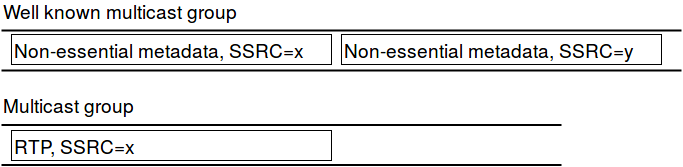
\includegraphics[width=\textwidth]{figures/non-essential-ssrc}
	\caption{The figures shows the well known multicast group and a data multicast group. In the well known multicast group, the non-essential metadata is sent with SSRC set to X, which is the same SSRc as in the data multicast group.}
\end{figure}





\subsection{Essential Metadata} \label{sec:design:essentalmetadata}
\textit{R1: Metadata must unambiguously relate to the streams.}\\
As described in section \ref{sec:design:sdp}, the SDP format specifies the multicast group of the actual data stream and those parameters that are needed in order to identify and decode to stream.
The essential metadata must therefore consist of at least those parameters required by the SDP format.\\

\noindent \textit{R2: Essential metadata must comprise hierarchical key-value pairs.}\\
The SDP protocol is key-value pairs which supports adding non-default key-value pairs as needed. \\

\noindent \textit{R3: Essential metadata must be retransmitted periodically}\\
In order to retransmit the essential metadata, the SDP packet must be sent periodically. How often the SDP packet is resent determines how long time \program{Subscribers} must wait before it has received a session announcement for all \program{Publishers}. If more often the session announcement is sent, the more bandwidth the session announcement will consume. A SDP file consumes around 300 bytes\footnote{Found by counting number of bytes of SDP example in SDP's RFC}. If the SDP is sent at 10 hz, it consumes 3Kb/s which is not critical compared to bandwidth consumed of a data stream of 6Mb/s. The refresh rate must be a parameter to the \program{Publisher}. \\

\noindent \textit{R4: The Essential metadata must contain a timestamp that relates to the sample number. The precision of the timestamp must be within the sample period}\\
By using the 64 bit NTP timestamp in the RTCP SR packet, the samples can be timestamped with a precision of 232 picoseconds\citep{RFC5905} which is sufficient.



\subsection{Software Components}
Due to design requirement X1, each program should do one thing and do it well.
In order to implement this, the functionality of the system has been split into four programs, namely: \pub{}, \sub{}, \pro{} and \con{}. The responsibility of each program is described below:

\begin{itemize}
	\item \pro: Is responsible for providing essential metadata, non-essential metadata and the source stream to the \pub.
	
	\item \pub: Is responsible for being the interface to the streams in a transparent manner, in order to hide the streams to the \pro. 
	
	\item \sub: Is responsible for subscribing to a stream and provide the source stream to the consumer. As with the \pub, the \sub is transparent meaning the \con is not aware of the streams. 
	
	\item \con: Is responsible for consuming the essential metadata, non-essential metadata and source stream.
\end{itemize}

The dataflow between the four programs is depicted in figure \ref{fig:design:pubsub}.
\begin{figure}[H]
	\centering
	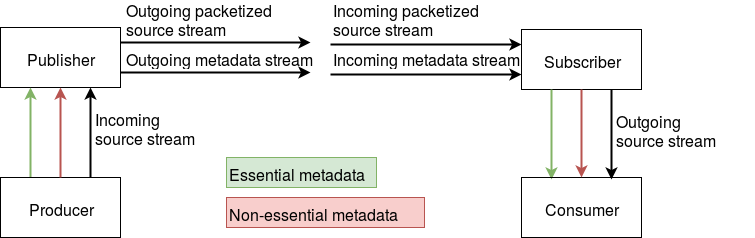
\includegraphics[width=1\textwidth]{figures/publisher-subscriber}
	\caption{ok} \label{fig:design:pubsub}
\end{figure}


Given design requirement X, it has been decided to interface the \pubs and \subs with the \pros{} and \cons{} using pipes, as this loosely couples the two pair of programs. Two pipes must be used, as the \pros{} and \subs{} must send a source stream and metadata to the \pubs{} and \cons, respectively.

\subsubsection*{Runmode}
In order to decide how the \pubs{} and \subs{} should be run with the \pros{} and \cons{}, three ideas are compared:
\begin{enumerate}
	\item \cons{} and \pros{} are logic master, to provide pipes to the \pubs{} and \subs{}. This requires the \cons{} and \pros{} to be made aware of the \subs{} and \pubs{}. 
	\item \subs{} and \pubs{} are logic master, and they provide handles to the \cons{} and \subs{}.
	\item \subs{} and \pubs{} are in a pipeline with the respective \cons{} and \pros{}, with non of the programs to be the logical masters. A fifth program have to be introduced that provides the pipes between the publisher/subscriber and the consumer/producer.
\end{enumerate}

From design requirement X(Unix, modularity), the programs should be encapsulated, meaning the \pubs{} and \subs{} must be opaque from the \cons{} and \pros{} respectively. As idea 1 requires the \cons{} and \pros{} to be the logical masters and thereby run the \pubs{} and \subs{}, this does not follow design requirement, as the producers and consumers must be aware of the publisher and subscribers.

Idea 3 is not considered, as it is unwanted to create a fifth program.

As idea 2 requires the \pubs{} and \subs{} to be the logical master of the \cons{} and \pros{}. This idea has been chosen, as this follow the design requirements X. This idea implies that the \pro{} is unaware about how handles the stream from the producer, and the consumer is unaware about who produces its input stream.  Idea 2 is depicted in figure \ref{fig:design:pubsub:runmode_master}.

\begin{figure}[H]
	\centering
	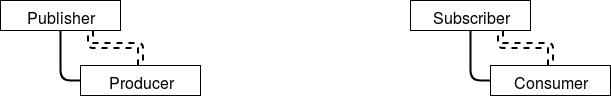
\includegraphics[width=1\textwidth]{figures/runmode_master}
	\caption{The figures shows the \pub{} and \sub{} are the logical master of the \pro{} and \con{} respectively. This design allows the \pubs{} to pass pipes to the \pro{} and \con{}, respectively} \label{fig:design:pubsub:runmode_master}
\end{figure}

\subsection{Publishers \& Subscribers}
From requirement P3, the \pub{} must single-handedly find an unused multicast group. In order for this to work without a designated master in the system, a session announcement mechanism must be designed which can be found in section \ref{sec:design:sessionannouncement}.


\noindent From requirement 1, a presence mechanism must be designed. This design is described in section \ref{sec:design:presencemechanism}. The design of the \pubs{} and \subs{} can be found in section \ref{sec:design:publisher} and \ref{sec:design:subscriber}, respectively.

As requirement 3 states, the \pubs{} and \subs{} must only run when 1) packets from a stream must be processed  2) when work must be done periodically. This requirement is similar to the general workflow of a \ac{GUI}, where code-blocks are executed when a button is clicked. These applications also usually implement timers such that code can be executed with a given interval. This is usually implemented in an event-driven manner where a method is attached to buttons and callbacks are attached to timers, such that the code can be run when the GUI either receives a click on a button from the user or the timer is invoked. \footnote{\url{https://en.wikipedia.org/wiki/Event-driven_programming}}

Given the nature of the \pubs{} and \subs{}, these two nodes should be implemented using event driven programming.


\subsubsection{Session Announcement} \label{sec:design:sessionannouncement}
Since multicast groups are chosen to distribute streams to multiple \subs, and the requirement that the \sub{} must not depend on too many wellknown multicast addresses, some algorithm must be design, that allows \subs{} to find the source streams, published by \pubs. As described in section \ref{sec:design:sap}, RTP sessions are announced using the SAP protocol with SDP on a wellknown multicast group. In order not to depend on an extra protocol, SAP is not used as it does not provide any additional features needed by the \pubs{} and \subs{}. Therefore, the SDP packets will simply be sent in an RTP session, on a wellknown multicast address where \subs{} can join to listen for session announcements. This is depicted in figure \ref{fig:design:pubsub:session_probe}.

\begin{figure}[H]
	\centering
	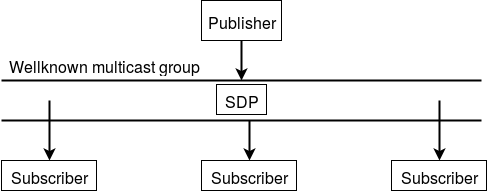
\includegraphics[width=1\textwidth]{figures/session-announcement-probe}
	\caption{The figure shows three \subs{} that probes the Wellknown multicast group, in order to know how the stream published by the \pub{}} \label{fig:design:pubsub:session_probe}
\end{figure}

A SDP packet then contains Essential metadata and an address to the multicast address of the source stream. When a \subs{} receives an SDP packet, it then knows which multicast group to join. This is depicted in figure \ref{fig:design:sessionannouncement}.

\begin{figure}[H]
	\centering
	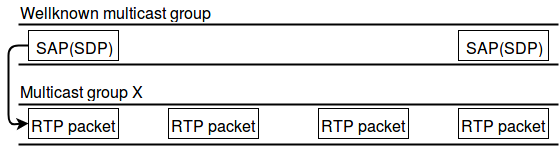
\includegraphics[width=\textwidth]{figures/sap-figure}
	 \caption{The figure shows a SDP packet is sent on a wellknown multicast group. The SDP contains essential metadata and announces the multicast group where the source stream can be found.}\label{fig:design:sessionannouncement}
\end{figure}


\subsubsection{Presence Mechanism} \label{sec:design:presencemechanism}
The presence mechanism can be implemented using the RTCP protocol. As mention in section \ref{sec:design:rtcp}, RTCP includes a SDES packet, that allows for identification of senders and receivers in an RTP session.
As it must take a maximum finite amounts of seconds to wait, the SDES  packet should be resent periodically. As the SDES packet is small(less than 100 bytes), no estimation of bandwidth is required. The default retransmission period must be a parameter on both \sub{} and \pub{}. RTCP also includes a BYE-packet, in order to inform other nodes that it is leaving a RTP session.
If a \program{Subscriber} or \program{Publisher} have not received a SDES packet from a \program{Publisher}/\program{Subscriber} for $2*\text{retransmission rate}$, it must be assumed that the \program{Subscriber}/\program{Publisher} is down and the BYE packet has been lost.
Given that RTCP packets are sent to an RTCP session, a \sub{} or \pub{} must join a particular RTP session, in order to get the RTCP packets and thereby information about who is present in a particular source stream. As all \pubs{} and \subs{} have joined the wellknown multicast group, the RTCP SDES packets should also be sent to the wellknown multicast group, such that all \pubs{} and \subs{} can see each other without being in the same source multicast group.

To summarize the packets that must be sent:
\begin{itemize}
	\item A RTCP bye packet must be sent when a \sub or \pub is leaving an RTP session.
	\item A RTCP SDES packet must be sent every X second containing CNAME of the host and whether it is a publisher or subscriber, to the well known multicast group and its source multicast group.
\end{itemize}



\subsubsection{Publisher} \label{sec:design:publisher}
From requirement 1b, the \pub{} must be able to single-handly find a free multicast group. To detect whether a multicast group is in use, can be handled by monitoring the well known address for $2*\text{SDP retransmission period}$ s. If a \program{Publisher} wants to send a source stream to multicast group X, it should join the wellknown multicast group in order to see if another \program{Publisher} announces a RTP session on multicast group X. If no session announcement of multicast group X is received, the \program{Publisher} can start sending announcements and send data to multicast group X. If a session announcement for multicast group X is received, the \program{Publisher} must generate a new multicast group, Y, where it again starts check if multicast group Y is in use. \footnote{It is known a race condition might occur if two \pubs{} join at the same time, this is discussed in section \ref{chp:discussion}} This is depicted in figure \ref{fig:design:pubsub:inuse}.

\begin{figure}[H]
	\centering
	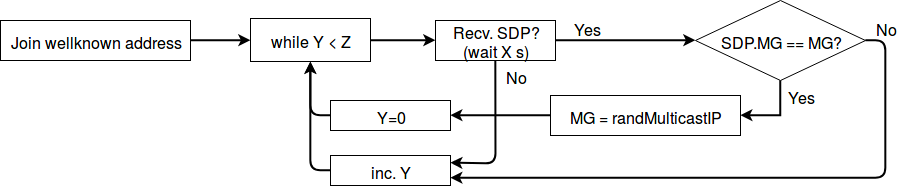
\includegraphics[width=\textwidth]{figures/flowchart-publisher-mg}
	\caption{The figure shows the flowchart of the mechanism to discover multicast groups in use.} \label{fig:design:pubsub:inuse}
\end{figure}


\myparagraph{Events}
Given that the \pub{} should be implement using in an event driven manner, the \pub{} must at least implement the following events:

\todo{Mention SR packet, track timerequirement from usecase -> analysis -> design.}

\begin{itemize}
	\item When an RTP packet is received from the wellknown multicast group.
	\item When a packet is received from the source stream from the \con{}.
	\item When a packet is received from the metadata stream from the \pro{}.
	\item When an RTCP SDES packet is received from the source stream.
	\item A timer to send RTCP SDES packets.
	\item A timer to send an RTCP SR packet.
	\item A timer to send SDP packets.
\end{itemize}

\todo{Publisher must support session announcement mechanism}
\subsubsection{Subscriber} \label{sec:design:subscriber}
From requirement R1 + R4, the \sub{} should be able to subscribe to a multicast group identified by a unique name of the stream. Since source multicast groups are announced using the Session Announcement mechanism described in section \ref{sec:design:sessionannouncement}, the \sub{} must support the mechanism. As source streams are sent as RTP streams, the \sub{} should support parsing the RTP packets form RTP streams. Using the two pipes from the \sub{} to the \con{}, the subscriber should write the source stream to one of the pipes, and non-essential as well as essential metadata to the other pipe.

\myparagraph{Events}
As with the \pub{}, the \sub{} must also implement an event loop. The \sub{} should at least implement the following events:

\begin{itemize}
	\item When an SDP packet is received from the wellknown multicast group.
	\item When an RTP packet is received from the source stream multicast group.
	\item When an RTCP packet is received from the source multicast group.
	\item A timer to send RTCP SDES packets.
\end{itemize}



\section{Historian}



\input{sections/impl_requirements}